\chapter{Quantum Field Theory}

    The main reference for this chapter is~\citet{peskin_introduction_1995}. For the section on the Connes--Kreimer algebra, see the original paper by~\citet{connes_hopf_1998} or the paper by~\citet{ebrahimi-fard_hopf_2005}. Another good reference on the formal structure of Feynman diagrams is~\citet{yeats_combinatorial_2017}. The main references for the section on entanglement are~\citet{tuybens_entanglement_2017,rangamani_holographic_2017}.

    \minitoc

\section{Klein--Gordon field}\index{Klein--Gordon equation}
\subsection{Lagrangian and Hamiltonian}

    The `simplest' Lagrangian (density) is given by
    \begin{gather}
        \label{qft:klein_gordon_lagrangian}
        \mathcal{L} = \frac{1}{2}\partial_\mu\phi\partial^\mu\phi - \frac{1}{2}m^2\phi^2\,.
    \end{gather}
    Using the principle of least action, the following Euler--Lagrange equation is obtained:
    \begin{gather}
        \left(\partial^\mu\partial_\mu + m^2\right)\phi = 0\,.
    \end{gather}
    This can be rewritten using the \textbf{d'Alembertian} $\Box = \partial_\mu\partial^\mu$:\index{d'Alembert!operator}
    \begin{gather}
        \label{qft:klein_gordon_equation}
        (\Box+m^2)\phi = 0\,.
    \end{gather}
    This equation is called the \textbf{Klein--Gordon equation}. In the limit $m\longrightarrow0$, this equation reduces to the well-known wave equation (\cref{optics:wave_equation}).

    From the Lagrangian~\eqref{qft:klein_gordon_lagrangian}, one can also derive a Hamiltonian function using \cref{classic:conjugate_momentum} and \cref{classic:hamiltonian}:
    \begin{gather}
        \label{qft:klein_gordon_hamiltonian}
        H = \frac{1}{2}\Int_{\mathbb{R}^3}\left[\pi^2(x) + (\nabla\phi(x))^2 + m^2\phi^2(x)\right]\,d^3x\,.
    \end{gather}

\subsection{Raising and lowering operators}

    Fourier transforming the scalar field $\phi(\symbf{x})$ and inserting it into the Klein--Gordon equation gives
    \begin{gather}
        \left(\partial_t^2+p^2+m^2\right)\phi(\symbf{p}) = 0\,.
    \end{gather}
    This is the equation for a simple harmonic oscillator with frequency $\omega = \sqrt{p^2+m^2}$.

    Analogous to ordinary quantum mechanics, raising and lowering operators $a_{\vector{p}}^\dag$ and $a_{\vector{p}}$ can be defined such that
    \begin{align}
        \phi(\vector{x}) &= \Int_{\mathbb{R}^3}\frac{d^3p}{(2\pi)^{3/2}}\frac{1}{\sqrt{2\omega_{\vector{p}}}}\left(a_{\vector{p}}e^{i\vector{p}\cdot\vector{x}} + a_{\vector{p}}^\dag e^{-i\vector{p}\cdot\vector{x}}\right)\,,\label{qft:phi}\\
        \pi(\vector{x}) &= \Int_{\mathbb{R}^3}\frac{d^3p}{(2\pi)^{3/2}}(-i)\sqrt{\frac{\omega_{\vector{p}}}{2}}\left(a_{\vector{p}}e^{i\vector{p}\cdot\vector{x}} - a_{\vector{p}}^\dag e^{-i\vector{p}\cdot\vector{x}}\right)\,.
    \end{align}
    An equivalent definition is obtained by performing the transformation $\vector{p}\longrightarrow-\vector{p}$ in the second term of $\phi(\vector{x})$ and $\pi(\vector{x})$:
    \begin{align}
        \phi(\vector{x}) &= \Int_{\mathbb{R}^3}\frac{d^3p}{(2\pi)^{3/2}}\frac{1}{\sqrt{2\omega_{\vector{p}}}}\left(a_{\vector{p}} + a_{-\vector{p}}^\dag\right)e^{i\vector{p}\cdot\vector{x}}\,,\\
        \pi(\vector{x}) &= \Int_{\mathbb{R}^3}\frac{d^3p}{(2\pi)^{3/2}}(-i)\sqrt{\frac{\omega_{\vector{p}}}{2}}\left(a_{\vector{p}} - a_{-\vector{p}}^\dag\right)e^{i\vector{p}\cdot\vector{x}}\,.
    \end{align}

    When the commutation relation
    \begin{gather}
        \label{qft:ladder_comutation}
        [a_{\vector{p}},a_{\vector{q}}^\dag] := \delta(\vector{p}-\vector{q})
    \end{gather}
    is imposed, the following commutation relation for the scalar field and its conjugate momentum is obtained:
    \begin{gather}
        [\phi(\vector{x}),\pi(\vector{y})] = i\delta(\vector{x} - \vector{y})\,.
    \end{gather}
    Now, the Hamiltonian can be calculated explicitly:
    \begin{gather}
        \label{qft:Klein_gordon_hamiltonian}
        H = \Int_{\mathbb{R}^3}\frac{d^3p}{(2\pi)^3}\omega_{\vector{p}}\left(a_{\vector{p}}^\dag a_{\vector{p}} + \frac{1}{2}[a_{\vector{p}},a_{\vector{p}}^\dag]\right)\,.
    \end{gather}
    However, it is clear from \cref{qft:ladder_comutation} that the second term in this integral diverges. There are two reasons for this divergence. First, space is infinite, i.e.~the $d^3x$ integral in \cref{qft:klein_gordon_hamiltonian} diverges. This problem can be resolved by restricting the system to a (finite) part of space or by considering the energy density instead of the energy itself. Second, by including very large values for $p$ in the integral, a parameter range is explored where the theory is likely to break down. To resolve this problem a  `high $p$'-cut-off should be introduced. A more practical solution, however, is to note that only energy differences are physical and so one can simply drop the second term altogether as it is merely a `constant' (albeit an infinite one).

    A corollary of \cref{qft:Klein_gordon_hamiltonian} together with the canonical commutation relations is
    \begin{align}
        [H,a_{\vector{p}}^\dag] &= \omega_pa_{\vector{p}}^\dag\,,\\
        [H,a_{\vector{p}}] &= -\omega_pa_{\vector{p}}\,.
    \end{align}
    As was the case for the quantum harmonic oscillator, the creation and annihilation operators deserve their names and one can write:
    \begin{gather}
        \ket{\vector{k}_1,\ldots,\vector{k}_n} = a^\dag(\vector{k}_1)\cdots a^\dag(\vector{k}_n)\ket{0}\,.
    \end{gather}
    Furthermore, this equation together with the canonical commutation relations imply that the Klein--Gordon fields are bosonic fields. This way of generating the full Hilbert (or, in fact, Fock) state space is axiomatized by the GNS construction (\cref{operators:gns}), where the vacuum plays the role of cyclic vector.

\subsection{Scalar propagator}

    \newformula{Pauli--Jordan function}{\index{Pauli--Jordan function}
        \begin{gather}
            i\Delta(\symbf{x}-\symbf{y}) := i[\phi(\symbf{x}),\phi(\symbf{y})] = \Int_{\mathbb{R}^3}\frac{d^3p}{(2\pi)^3}\frac{1}{2\omega_{\symbf{x}}}\left(e^{-i\symbf{p}\cdot(\symbf{x}-\symbf{y})} - e^{i\symbf{p}\cdot(\symbf{x}-\symbf{y})}\right)
        \end{gather}
        When $x^0=y^0$ (ETCR) or $(\symbf{x}-\symbf{y})^2 < 0$ (spacelike curves), the Pauli--Jordan function is identically 0. (See also the \textit{axiom of microcausality}~\ref{aqft:microcausality}).
    }

\subsection{Normalization constant}

    By \cref{distribution:delta_of_function}, the delta function $\delta^{(3)}(\vector{p}-\vector{q})$ transforms as $\delta^{(3)}(\Lambda\vector{p} - \Lambda\vector{q})\frac{\Lambda E}{E}$ under a general Lorentz boost $\Lambda$. Although this is clearly not Lorentz invariant, the quantity $E_{\symbf{x}}\delta^{(3)}(\vector{p}-\vector{q})$ can be seen to be invariant. From this observation it follows, that the correct normalization in the momentum representation is
    \begin{gather}
        \ket{\symbf{p}} = \sqrt{2E_{\symbf{x}}}a_{\symbf{p}}^\dag\ket{0}
    \end{gather}
    and, hence,
    \begin{gather}
        \langle\symbf{p}\mid\symbf{q}\rangle = 2E_{\symbf{x}}(2\pi)^3\delta^{(3)}(\vector{p}-\vector{q})\,,
    \end{gather}
    where the constants are a matter of convention to cancel the constants in \cref{qft:phi}.

\subsection{Invariant integration measure}

    The factor $2E_p$ does not only occur in the normalization conditions. To find a Lorentz-invariant integration measure in spacetime, the following integral can be studied:
    \begin{gather}
        \Int_{\mathbb{R}^3}\frac{d^3p}{2E_p} = \Int_{\mathbb{R}^+\times\mathbb{R}^3}\delta(p^2-m^2)\,d^4p\,,
    \end{gather}
    where the timelike component $p^0$ is restricted to be (strictly) positive. By using this measure, it is ensured that the integral of any Lorentz-invariant function is again Lorentz invariant.
    \begin{example}[One-particle identity operator]\index{identity!operator}
        \begin{gather}
            \mathbbm{1} := \Int_{\mathbb{R}^3}\frac{d^3p}{2E_p}\ket{\symbf{p}}\bra{\symbf{p}}
        \end{gather}
    \end{example}

\section{Contractions and Wick's theorem}
\subsection{Bosonic fields}

    In the following definitions, (field) operators will be decomposed as \[\phi = \phi^{(+)} + \phi^{(-)}\,,\] where the + symbol denotes the `positive-frequency' part, i.e.~the part consisting of annihilation operators. The `negative-frequency' part is defined analogously. This terminology stems from classic Fourier theory. By looking at \cref{qft:phi} and remembering that the $(1,3)$-signature is adopted, the annihilators can be seen to always occur together with a positive-frequency exponential.

    \newdef{Contraction for neutral bosonic fields}{\index{contraction}
        \begin{gather}
            \contraction{}{\phi}{(\symbf{x})}{\phi}\phi(\symbf{x})\phi(\symbf{y}) :=
            \begin{cases}
                [\phi(\symbf{x})^{(+)},\phi(\symbf{y})^{(-)}]&\cif x^0>y^0\\
                [\phi(\symbf{y})^{(+)},\phi(\symbf{x})^{(-)}]&\cif y^0>x^0
            \end{cases}
        \end{gather}
    }
    \newformula{Feynman propagator}{\index{Feynman!propagator}\label{qft:feynman_propagator_contraction}
        \begin{gather}
            i\Delta_F(\symbf{x}-\symbf{y}) := \contraction{}{\phi}{(\symbf{x})}{\phi}\phi(\symbf{x})\phi(\symbf{y}) := i\lim_{\varepsilon\rightarrow 0^+}\Int_{\mathbb{R}^4}\frac{d^4p}{(2\pi)^4}\frac{e^{-i\symbf{p}\cdot(\symbf{x}-\symbf{y})}}{p^2 - m^2 + i\varepsilon}
        \end{gather}
    }

    \newdef{Contraction for charged bosonic fields}{
        \begin{gather}
            \contraction{}{\phi}{(\symbf{x})}{\overline\phi}\phi(\symbf{x})\overline\phi(\symbf{y}) :=
            \begin{cases}
                [\phi(\symbf{x})^{(+)},\overline\phi(\symbf{y})^{(-)}]&\cif x^0>y^0\\
                [\phi(\symbf{y})^{(+)},\overline\phi(\symbf{x})^{(-)}]&\cif y^0>x^0
            \end{cases}
        \end{gather}
    }

    \newdef{Normal ordering}{\index{normal!ordering}\label{qft:normal_ordering}
        The normal ordering $\mathcal{N}$, often denoted by colons $:\ \ :$, of a sequence of field operators is defined as the permuted sequence in which all annihilation operators appear on the right of the creation operators, e.g.:
        \begin{gather}
            \mathcal{N}\bigl(\phi(\symbf{x})\phi^\dag(\symbf{y})\phi(\symbf{z})\bigr) = \phi^\dag(\symbf{y})\phi(\symbf{x})\phi(\symbf{z})\,.
        \end{gather}
        Note that the normal ordering operator is not a morphism between CCR-algebras since this would lead to a contradiction:
        \begin{gather}
            b_ib_j^\dag = b_j^\dag b_i + \delta_{ij}\implies\mathcal{N}(b_ib_j^\dag) = \mathcal{N}(b_j^\dag b_i+\delta_{ij}) = \mathcal{N}(b_j^\dag b_i) + \delta_{ij}\implies\delta_{ij}=0\,.
        \end{gather}
        The solution is given by the fact that inside the normal ordering all operators commute and, hence, this ordering can be axiomatized as an algebra morphism $\mathcal{N}:\Sym^\bullet A\rightarrow A$, where $A$ is the CCR-algebra of the theory (see~\citet{miwa_solitons_2000}).
    }
    \begin{property}
        From this definition, it immediately follows that the vacuum expectation value of a normal ordered sequence is 0.
    \end{property}

    \newformula{Wick's theorem for bosonic fields}{\index{Wick}
        \begin{gather}
            \mathcal{T}\bigl(\phi(\symbf{x}_1)\cdots\phi(\symbf{x}_n)\bigr) = \mathcal{N}\bigl(\phi(\symbf{x}_1)\cdots\phi(\symbf{x}_n) + \text{all possible contractions}\bigr)
        \end{gather}
        When acting with a time-ordered product on the vacuum, this relation implies that only fully contracted terms will remain. Moreover, by \cref{qft:feynman_propagator_contraction}, every such action can be expressed solely in terms of propagators.
    }

    \begin{remark}
        In the case of charged bosons, only contractions of the form $\contraction{}{\phi}{(\symbf{x})}{\overline\phi}\phi(\symbf{x})\overline\phi(\symbf{y})$ will remain because $[a,b^+]=0$.
    \end{remark}

    \begin{result}
        \begin{gather}
            \contraction{}{\phi}{(\symbf{x})}{\phi}\phi(\symbf{x})\phi(\symbf{y}) = \mathcal{T}\bigl(\phi(\symbf{x})\phi(\symbf{y})\bigr) - \mathcal{N}\bigl(\phi(\symbf{x})\phi(\symbf{y})\bigr)
        \end{gather}
    \end{result}

    Wick's theorem has an analogue in probability theory.
    \begin{theorem}[Isserlis]\index{Isserlis}
        Let $X_1,\ldots,X_n$ be a set of random variables following a multinormal distribution with mean 0.
        \begin{gather}
            \expect{X_1\cdots X_n} = \sum_{\sigma\in P_{n,2}}\prod_{\{i,j\}\in\sigma}\expect{X_iX_j}\,,
        \end{gather}
        where $P_{n,2}$ denotes the set of binary partitions of $\{1,\ldots,n\}$. Because the mean of the distribution is zero, this expression is equal to
        \begin{gather}
            \expect{X_1\cdots X_n} = \sum_{\sigma\in P_{n,2}}\prod_{\{i,j\}\in\sigma}\mathrm{cov}\bigl[X_i,X_j\bigr]\,.
        \end{gather}
    \end{theorem}

\subsection{Fermionic fields}

    \newdef{Contraction}{
        \begin{gather}
            \contraction{}{\psi}{(\symbf{x})}{\overline\psi}\psi(\symbf{x})\overline\psi(\symbf{y}) :=
            \begin{cases}
                \{\psi(\symbf{x})^{(+)},\overline\psi(\symbf{y})^{(-)}\}_+&\cif x^0>y^0\\
                -\{\psi(\symbf{y})^{(+)},\overline\psi(\symbf{x})^{(-)}\}_+&\cif y^0>x^0
            \end{cases}
        \end{gather}
    }
    \begin{remark}
        Only contractions of the form $\contraction{}{\psi}{(\symbf{x})}{\overline\psi}\psi(\symbf{x})\overline\psi(\symbf{y})$ will remain because $\{a,b^\dag\}_+=0$.
    \end{remark}

    \newformula{Feynman propagator}{\index{Feynman!propagator}
        \begin{gather}
            i\Delta_F(\symbf{x}-\symbf{y}) := \contraction{}{\psi}{(\symbf{x})}{\overline\psi}\psi(\symbf{x})\overline\psi(\symbf{y}) := i\lim_{\varepsilon\rightarrow 0^+}\Int_{\mathbb{R}^4}\frac{d^4\symbf{p}}{(2\pi)^4}\frac{\slashed{\symbf{p}} + m}{p^2 - m^2 + i\varepsilon}e^{-i\symbf{p}\cdot(\symbf{x}-\symbf{y})}
        \end{gather}
    }

    \begin{remark}[Normal ordering]\label{qft:ordering_morphism}
        One should take into account the Fermi--Dirac statistics when permuting fermionic field operators under a normal ordering. A general factor $\sgn(\sigma)$, where $\sigma$ is the permutation of the operators, will arise in every term, e.g.:
        \begin{gather}
            \mathcal{N}\bigl(\psi(\symbf{x})\overline\psi(\symbf{y})\psi(\symbf{z})\bigr) = -\overline\psi(\symbf{y})\psi(\symbf{x})\psi(\symbf{z})\,.
        \end{gather}
        A similar remark should be made for the time-ordering operator $\mathcal{T}$. As was the case for bosonic theories (\cref{qft:normal_ordering}), one should pay attention to the nature of the normal ordering. It is not a morphism between CAR-algebras, but instead it is an algebra morphism between a free (odd) algebra and a CAR-algebra.
    \end{remark}

\section{Gauge theory}\label{section:qft_gauge_theory}

    In this section, the theories from \cref{chapter:constrained_dynamics,chapter:gauge_theory} will be quantized. Due to the gauge invariance and, hence, the redundancies in the fields, the path integral diverges. Several solutions exist, ranging from rather ad-hoc procedures (as described first) to very general methods. The general gauge structure of Lagrangian (field) theories was considered in \cref{chapter:constrained_dynamics}. The resulting structure was the BV-BRST complex, which gives a homological resolution of both the critical locus of the field equations and the gauge orbits of the gauge symmetries. The main object was a gauge-invariant action and an extended covariant phase space containing both fields and antifields with the structure of a symplectic dg-manifold (\cref{hdg:dg_symplectic_manifold}). The quantum analogue of this structure will be discussed below.

\subsection{Schwinger--Dyson equation}\index{Schwinger--Dyson equation}

    Consider the following path-integral representation of the expectation value of a (polynomially bounded) functional $F$:\footnote{The normalization factor has been left out for convenience.}
    \begin{gather}
        \langle F\rangle = \Int F[\phi]\exp\left(i/\hbar S[\phi]\right)\,D\phi\,.
    \end{gather}
    If the field measure $D\phi$ is an appropriate generalization of the Lebesgue/Haar measure on $\mathbb{R}^n$, it is invariant under translations $\phi\longrightarrow\phi+\xi$.\footnote{This is, for example, not the case for nonlinear $\sigma$-models, where the target space is a manifold and not a vector space.} It follows that the expectation value is also given by
    \begin{gather}
        \langle F\rangle = \Int F[\phi+\xi]\exp\left(i/\hbar S[\phi+\xi]\right)\,D\phi\,.
    \end{gather}
    Equating these two expressions and expanding to first order gives the Schwinger--Dyson equations:
    \begin{gather}
        \label{qft:schwinger_dyson_equations}
        \left\langle\frac{\delta^LF}{\delta\phi^I}\right\rangle = -i\hbar\left\langle\frac{\delta^LS}{\delta\phi^I}F\right\rangle
    \end{gather}
    for all $I\in\mathcal{I}$. This can be recast in geometric form through \cref{constraint:antifield_vector_field}. A polynomial functional that is linear in antifields is of the form $\lambda^I\mathcal{P}_I$. Geometrically, this corresponds to the vector field
    \begin{gather}
        X_\lambda = \lambda^I\frac{\delta^L}{\delta\phi^I}\,.
    \end{gather}
    The Schwinger--Dyson equation then becomes
    \begin{gather}
        \mathcal{T}\left(\mathcal{L}_{X_\lambda}e^{i/\hbar S[\phi]}\right)=0\,.
    \end{gather}
    
    \begin{remark}[Nonperturbative QFT]
        The Schwinger--Dyson equations can be taken as the fundamental starting point of QFT for a nonperturbative approach.
    \end{remark}

    Note that, even on shell, the time-ordered product $\mathcal{T}\left(F\frac{\delta S}{\delta\phi}\right)$ does not generally vanish. However, when $F$ has a different spacetime support than $\phi$, there is no operator-ordering issue and, accordingly, the expectation value does vanish. As such, the equations of motion can be seen to hold quantum mechanically away from the diagonal.

    \begin{property}[Observable equivalence]
        Classically, two functionals $F,G$ are said to be equivalent on shell whenever
        \begin{gather}
            F-G \approx 0
        \end{gather}
        or, equivalently (\cref{constraint:weakly_vanishing_functions}),
        \begin{gather}
            F-G = \frac{\delta^LS}{\delta\phi^I}\lambda^I
        \end{gather}
        Note that the DeWitt convention~\eqref{constraint:dewitt_convention} is used here. Through the Schwinger--Dyson equation, this can be extended to QFTs:
        \begin{gather}
            F\sim G\iff F-G = \frac{\delta^LS}{\delta\phi^I}\lambda^I-i\hbar\frac{\delta^L\lambda^I}{\delta\phi^I}\,.
        \end{gather}
        Two functionals in the same \textbf{quantum equivalence class} will have the same expectation value. Note that, for $\hbar\longrightarrow0$, this recovers the classical situation. In this way, the Schwinger--Dyson equation also characterizes the kernel of the time-ordering operator $\mathcal{T}$ sending (classical) off-shell observables to (quantum) on-shell observables (cf.~\cref{qft:ordering_morphism}).
    \end{property}

    In \cref{section:BV_formalism}, it was shown how the classical equivalence of functionals can be implemented homologically through the BV-BRST complex. Of course, the question arises whether the quantum equivalence relation can also be resolved in a similar way. An essential property of the antibracket was that it constituted a (graded) derivation. However, because of quantum corrections, the quantum BRST operator $\mathcal{S}$ cannot be a derivation. The product of $\mathcal{S}$-exact will not, in general, be $\mathcal{S}$-exact, since $\langle A\rangle = 0 = \langle B\rangle$ does not imply $\langle AB \rangle=0$ (in fact, it is $\langle AB \rangle\sim\hbar$).

\subsection{Faddeev--Popov integration}\index{Faddeev--Popov!integral}

    Introducing ghost variables is not only useful for obtaining a resolution of the gauge orbits. It also helps with path integral quantization of gauge theories, where it removes divergences from the path integral. (Of course, this boils down to the same purpose, since the divergence arise from overcounting gauge orbits.)

    First, consider a classical theory with second-class constraints. These can be taken care of by passing from the Poisson bracket to the Dirac bracket (\cref{constraint:dirac_bracket}). With respect to a triangulation of the path integral, one, hence, has to replace the ordinary Liouville measure by a modified version:
    \begin{gather}
        \Int\prod_{\symbf{x}}\mathrm{Ber}(\sigma_{ij})^{1/2}\exp\bigl(i/\hbar S[\phi]\bigr)[D\phi]\,,
    \end{gather}
    where $\sigma_{ij}$ is the structure matrix of the Dirac bracket and $\mathrm{Ber}$ denotes the Berezinian (\cref{hda:berezinian}). In terms of the constraint matrix $C_{ab}=\{\chi_a,\chi_b\}$, this becomes:
    \begin{gather}
        \Int\prod_{a,\symbf{x}}\delta(\chi_a)\mathrm{Ber}(C_{ab})^{1/2}\exp\bigl(i/\hbar S[\phi]\bigr)[D\phi]\,.
    \end{gather}

    For first-class constraints, the approach is slightly different and one needs to construct the reduced phase space. (From now on, it is assumed that there are no second-class constraints left.) Consider a complete set of variables $\widetilde{z}^\alpha$ with their associated structure matrix $\sigma^{\alpha\beta}:=\{\widetilde{z}^\alpha,\widetilde{z}^\beta\}$. The reduced path integral is
    \begin{gather}
        \Int\prod_{\symbf{x}}\mathrm{Ber}(\sigma_{\alpha\beta})^{1/2}\exp\bigl(i/\hbar S[\widetilde{z}]\bigr)[D\widetilde{z}]\,,
    \end{gather}

    \begin{remark}[Gribov ambiguity]
        The reduced path integral is gauge invariant and, more importantly, requires no gauge-fixing conditions. Accordingly, it does not suffer from the Gribov problem (\cref{gauge:gribov_ambiguity}).
    \end{remark}

    To obtain the reduced variables $\widetilde{z}$ is a difficult and, possibly, impossible task. However, sometimes, there exist gauge conditions $\chi_a=0$ that carve out the reduced phase space. The combined constraints $\chi_\alpha\equiv(G_a,\chi_a)$ are always second class. Moreover, the Berezinian satisfies
    \begin{gather}
        \mathrm{Ber}\bigl(\{\chi_\alpha,\chi_\beta\}\bigr) = \mathrm{Ber}\bigl(\{G_a,\chi_b\}\bigr)\,.
    \end{gather}
    The reduced path integral can, hence, be rewritten as
    \begin{gather}
        \Int\prod_{\symbf{x}}\delta(\chi)\delta(G)\mathrm{Ber}\bigl(\{G_a,\chi_b\}\bigr)\exp\bigl(i/\hbar \widetilde{S}[z]\bigr)[Dz]\,,
    \end{gather}
    where $\widetilde{S}$ contains the boundary term $M$ in \cref{constraint:symplectic_potential}. Introducing Fourier transforms recovers (part of) \cref{constraint:FP_action}:
    \begin{gather}
        \Int\prod_{\symbf{x}}\delta(\chi)\exp\frac{i}{\hbar}\left(\widetilde{S}[z]-\Int v^aG_a\vol_M-\Int\overline{C}\vphantom{C}^b\delta_C\chi_b\vol_M\right)[Dz][Dv][DC][D\overline{C}]\,.
    \end{gather}
    This is the \textbf{Faddeev--Popov path integral} and the $C,\overline{C}$ are the \textbf{Faddeev--Popov ghosts}.\index{Faddeev--Popov!path integral}\index{Faddeev--Popov!ghost}

\subsection{BV-BRST theory}

    \newdef{BV Laplacian}{\index{Batalin--Vilkovisky!Laplacian}
        Consider a BV manifold $(M,\omega,S)$. A BV Laplacian is an operator $\Delta$ that satisfies the following conditions:
        \begin{enumerate}
            \item\textbf{Nilpotency}: $\Delta^2=0$, and
            \item\textbf{Product rule}: $\Delta(fg)= (\Delta f)g + (-1)^{\varepsilon(f)}f(\Delta g) + (-1)^{\varepsilon(f)}(f,g)$,
        \end{enumerate}
        where $(\cdot,\cdot)$ is the induced Poisson/Gerstenhaber bracket. Although $\Delta$ is not a derivation with respect to ordinary multiplication --- the product rule says that the bracket measures the deviation of $\Delta$ from being a derivation --- these relations do imply that the BV Laplacian acts as a graded derivation with respect to the bracket:
        \begin{gather}
            \Delta(f,g) = (\Delta f,g) + (-1)^{\varepsilon(f)+1}(f,\Delta g)\,.
        \end{gather}
        The canonical BV Laplacian in field-antifield coordinates is given by (the DeWitt convention is still used here)
        \begin{gather}
            \Delta_{\text{BV}} := (-1)^{\varepsilon_I+1}\frac{\partial^R}{\partial\phi^I}\frac{\partial^R}{\partial\mathcal{P}_I} + (-1)^{\varepsilon_a+1}\frac{\partial^R}{\partial\eta^a}\frac{\partial^R}{\partial\mathcal{P}_a}\,.
        \end{gather}
    }

    For functionals that are linear in antifields\footnote{Terms of higher order can be reduced to this case through the product rule.}, the BV Laplacian recovers the correction term in the Schwinger--Dyson equations:
    \begin{gather}
        \Delta\left(\mathcal{P}_I\lambda^I[\phi]\right) = (-1)^{\varepsilon(\lambda^I)-1}\frac{\delta^L\lambda^I}{\delta\phi^I}\,.
    \end{gather}
    Hence, the quantum-mechanical analogue of the BRST operator is
    \begin{gather}
        \mathcal{S}F := (F,S) - i\hbar\Delta F\,,
    \end{gather}
    where $S$ is the classical action. The BV Laplacian gives exactly the quantum corrections to the classical BRST operator.

    \begin{formula}[Schwinger--Dyson equations]\index{Schwinger--Dyson equation}
        For functionals that are linear in the antiields, i.e.~vector fields on the BV manifold, \cref{qft:schwinger_dyson_equations} can be rewritten as
        \begin{gather}
            \langle\mathcal{S}F\rangle = 0\,.
        \end{gather}
        For this reason, the quantum BRST operator is also called the \textbf{Schwinger--Dyson operator}.
    \end{formula}

    % \newformula{Quantum master equation}{\index{master equation!quantum}
    %     Let $S$ be the classical action. After quantization, the master equation~\ref{constraint:master_equation} becomes
    %     \begin{gather}
            
    %     \end{gather}
    % }
    \begin{formula}[Quantum master equation]\index{master equation}
        Consider the function $f:=e^{iS/\hbar}$ on a BV manifold $(M,\omega,S)$. Because
        \begin{gather}
            \Delta_{\text{BV}}f = \frac{i}{\hbar}\Delta S e^{iS/\hbar} + \left(\frac{i}{\hbar}\right)^2\frac{1}{2}(S,S)e^{iS/\hbar}\,,
        \end{gather}
        the condition that $f$ is BV-harmonic is equivalent to $S$ satisfying
        \begin{gather}
            \frac{1}{2}(S,S)-i\hbar\Delta_{\text{BV}}S=0\,.
        \end{gather}
        This equation is called the quantum master equation. Expanding $S$ as a power series in $\hbar$ shows that the order-0 term satisfies the classical master equation~\eqref{hdg:classical_master_equation}.
    \end{formula}

    \newdef{BV integral}{\index{Batalin--Vilkovisky!integral}\index{gauge!fixing}\index{integral|seealso{Batalin--Vilkovisky}}
        Consider the shifted cotangent bundle $\Pi T^*M$ on an $m$-dimensional smooth manifold. Let the gauge-fixing fermion $K$ be an odd function of the even coordinates of a Darboux basis (denote these coordinates by $q^i$). This function determines a projectable Lagrangian submanifold $L_K\subset\Pi T^*M$ by the Maslow--H\"ormander theorem~\ref{symplectic:maslow_hormander} given by
        \begin{gather}
            L_K = \left\{(q^i,p_i)\in\Pi T^*M\,\middle\vert\,p_i=\pderiv{K}{q^i}\right\}\,.
        \end{gather}
        The Batalin--Vilkovisky integral of a function $f\in C^\infty(M)$ with respect to $K$ is defined as
        \begin{gather}
            \Int_{L_K}f\sqrt{\vol_\omega}\,,
        \end{gather}
        where $\sqrt{\vol_\omega}$ is the volume form on Lagrangian submanifolds induced by $\omega$. The BV integral and BV Laplacian interact in the following way (for BV integrable $f$):
        \begin{enumerate}
            \item If $f=\Delta_{\text{BV}}g$, then $\int_{L_K}f = 0$ for all gauge-fixing fermions $K$.
            \item If $\Delta_{\text{BV}}f=0$, then $\displaystyle\deriv{}{t}\int_{L_{K_t}}f=0$, where $\{K_t\}_{t\in\mathbb{R}}$ is a continuous family of gauge-fixing fermions.
        \end{enumerate}
        The second property implies that the BV integral is invariant under deformations of the domain of integration.
    }

    \begin{property}[Divergence]\index{divergence}
        Consider a superdensity $\mu$ (or a volume form) on a BV manifold (any supermanifold actually suffices). This density induces a divergence on vector fields (i.e.~antifields) by generalizing \cref{riemann:divergence_partial}:
        \begin{gather}
            \mathrm{div}(F) := -\frac{1}{\mu}\frac{\delta^R}{\delta\phi^I}\left((-1)^{\varepsilon_I}\mu\frac{\delta^RF}{\delta\mathcal{P}_I}\right)\,.
        \end{gather}
        When $\mu=1$, one obtains $\div(F)=\Delta F$, i.e.~the BV Laplacian is exactly the divergence.
    \end{property}
    \begin{remark}[de Rham differential]
        The BV Laplacian can also be obtained as the dual to the de Rham differential when identifying $p$-vector fields with $(n-p)$-forms through the volume form.
    \end{remark}

\section{Quantum chromodynamics}\label{section:qcd}

	\newprop{OZI rule\footnotemark}{\index{OZI rule}
		\footnotetext{\textit{Okubo, Zweig} and \textit{Iizuka}}
		Decay processes for which the corresponding Feynman diagrams become disconnected (initial states and final states are disconnected) when removing internal gluon lines, are suppressed with respect to other processes.
	}

\section{Feynman rules}
\subsection{Scalar theory}

    By expanding the correlation functions in perturbation theory and applying Wick's theorem, one can rewrite every term using the following dictionary for Feynman diagrams (it is assumed that every coupling constant in the Lagrangian is divided by the necessary permutation factors, e.g.~in $\phi^4$-theory it is assumed that the constant is of the form $\lambda/4!$):
    \begin{itemize}
        \item Propagator $\Delta_F(\symbf{x}-\symbf{y})$:
            \begin{gather*}
                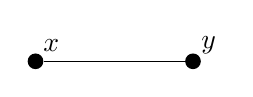
\begin{tikzpicture}
                    \node (labx) at (0.2,0.2) {$\symbf{x}$};
                    \node (laby) at (2.2,0.2) {$\symbf{y}$};
                    \node (x) at (0,0) [circle,fill,inner sep=2pt] {};
                    \node (y) at (2,0) [circle,fill,inner sep=2pt] {};
                    \draw (x) -- (y);
                \end{tikzpicture}
            \end{gather*}
        \item Interaction vertex\footnote{Four legs were drawn as an example but this can be generalized to any order of interaction term.} $-i\lambda\int d^4z$:
            \begin{gather*}
                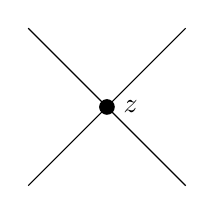
\begin{tikzpicture}
                    \node (z) at (0.3,0) {$z$};
                    \node (x) at (0,0) [circle,fill,inner sep=2pt] {};
                    \draw (-1,-1) -- (1,1);
                    \draw (-1,1) -- (1,-1);
                \end{tikzpicture}
            \end{gather*}
    \end{itemize}
    The main idea behind these rules is to draw all possible diagrams consistent with the given interaction Lagrangian and translate them into analytic expressions. However, to obtain the correct normalization, one should take the following remark into account.
    \begin{remark}\index{symmetry!factor}
        Symmetry factors of diagrams should be accounted for in analytic expressions. As an example, consider the following vacuum bubble:
        \begin{gather*}
            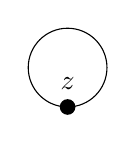
\begin{tikzpicture}
                \node (z) at (0, 0.3) {$z$};
                \node (x) at (0,0) [circle,fill,inner sep=2pt] {};
                \draw (0,0.5) circle (0.5);
            \end{tikzpicture}
        \end{gather*}
        Because the two legs can be interchanged, this diagram has \textbf{symmetry factor} 2 and, hence, it gives the analytic expression $-\frac{i\lambda}{2}\int d^4z\,\Delta_F(\symbf{z}-\symbf{z})$.
    \end{remark}

\subsection{Graph theory}\index{graph}

    Given a decorated graph $\Gamma$, representing a Feynman diagram, collapsing all vertices leads to its residue $\mathrm{res}(\Gamma)$. Such a one-vertex graph $\underline{r}$, where $r\in\mathbb{N}$ is the number or remaining edges, is sometimes also called the \textbf{external leg structure} of all graphs $\Gamma$ with $\mathrm{res}(\Gamma)=\underline{r}$. Two other important properties of a graph $\Gamma$ are its degree and its symmetry factor.

    \newdef{Degree}{\index{degree}
        Consider a graph $\Gamma$. Its degree $|\Gamma|\in\mathbb{N}$ is given by the number of independent loops in $\Gamma$ or, equivalently, the rank of its first homology group $H_1(\Gamma;\mathbb{Z})$ (\cref{topology:simplicial_homology_group}), i.e.~its first Betti number.
    }

    \newdef{1PI graph}{\index{graph!1PI}\index{irreducible!graph}
        A graph that remains connected when an internal edge is removed.
    }

    Several different ways exist to determine the number of relevant permutations of the Feynman diagram. One is to directly use Wick's theorem and get the combinatorics out of that result. However, two other useful approaches exist.
    \newdef{Symmetry factor}{\index{symmetry!factor}
        Consider a Feynman diagram $\Gamma$ consisting of $n\in\mathbb{N}$ internal vertices of valence $\nu\in\mathbb{N}_{\geq3}$.\footnote{It is here assumed that all vertices are of the same valence and type. The definition is easily extended to more complex diagrams.} The symmetry factor is given by:
        \begin{gather}
            \mathrm{sym}(\Gamma) := \frac{1}{n!}\left(\frac{1}{\nu!}\right)^nC\,,
        \end{gather}
        where $C\in\mathbb{N}$ denotes the number of different ways that the vertices can be contracted while resulting in the same diagram.
    }
    A more structured way is to consider the suitable notion of graph automorphism for Feynman diagrams. For ordinary graphs, two common definitions are either through an \textit{adjacency matrix} or through a relation on edges.\index{matrix!adjacency} A third, equivalent, way, however, is through the notion of `half-edge'.
    \newadef{Graph}{\index{graph}\index{half-!edge}\index{vertex}\index{edge}
        Consider a set of \textbf{half-edges} $\Gamma$. A graph structure on $\Gamma$ consists of a partition $\mathcal{E}$ by subsets of cardinality 2, called the \textbf{edge} set, and a partition $\mathcal{V}$, the \textbf{vertex} set.
    }
    By slightly modifying this definition, a Feynman diagram is obtained.
    \newadef{Symmetry factor}{\index{symmetry!factor}\index{Feynman!diagram}
        Consider a set of \textbf{half-edges} $\Gamma$. A Feynman diagram structure on $\Gamma$ consists of a disjoint collection $\mathcal{E}$ of cardinality-2 subsets, called the \textbf{internal edge} set, and a partition $\mathcal{V}$ by subsets of cardinality at least 3, the \textbf{vertex} set. Half-edges not part of the internal edge set are called external edges. These determine the residue $\mathrm{res}(\Gamma)$.

        An automorphism of a Feynman diagram consists of a bijection $\Gamma\rightarrow\Gamma$ that fixes the external edges and $\mathcal{E},\mathcal{V}$. The symmetry factor of $\Gamma$ is then given by:
        \begin{gather}
            \mathrm{sym}(\Gamma) = |\Aut(\Gamma)|\,.
        \end{gather}
    }

    Aside from the obvious algebra structure on Feynman diagrams, given by formal linear combinations and juxtaposition, there also exists a pre-Lie algebra structure (\cref{lie:pre_lie_algebra}):
    \begin{gather}
        \label{qft:pre_lie_algebra}
        (\Gamma_1,\Gamma_2) = \sum_\Gamma n(\Gamma_1,\Gamma_2;\Gamma)\Gamma\,,
    \end{gather}
    where $n(\Gamma_1,\Gamma_2;\Gamma)\in\mathbb{N}$ counts the number of ways that, if $\Gamma_2$ is a subgraph of $\Gamma$, $\Gamma/\Gamma_2\cong\Gamma_1$ and $\Gamma$ ranges over 1PI diagrams.

\subsection{Degree of divergence}

    \newdef{Mass dimension}{\index{dimension!mass}
        Through the de Broglie or Compton wavelengths, respectively \cref{qm:debroglie_wavelength} and \cref{qm:compton_wavelength}, the dimensions of length and mass are related. In particular, in natural units $\hbar=c=1$, one obtains $[m]=[\lambda]^{-1}$. This dimension is called the mass dimension.

        Now, consider a general Lagrangian density $\mathcal{L}$. Since this density is integrated against a volume form to obtain the dimensionless action, the mass dimension of $\mathcal{L}$ has to equal the spacetime dimension:
        \begin{gather}
            [\mathcal{L}] = d\,.
        \end{gather}
        To obtain the mass dimension of a field $\phi$, the general procedure, is to look at the mass term in the Lagrangian. For example, for scalar theories:
        \begin{align*}
            [\mathcal{L}_{\text{mass}}] &= \left[\frac{1}{2}m^2\phi^2\right]\\
            &= 2 + 2[\phi]
        \end{align*}
        and, hence
        \begin{gather}
            [\phi] = \frac{d-2}{2}\,.
        \end{gather}
    }

    \newdef{Degree of divergence}{\index{degree!of divergence}
        Consider a general Feynman diagram $\Gamma$ and its associated integral $I_\Gamma$. The (superficial) degree of divergence of $\Gamma$ is defined as
        \begin{gather}
            D_\Gamma := \text{power of momenta in numerator} - \text{power of momenta in denominator}\,.
        \end{gather}
        This can also be calculated at the level of the graph $\Gamma$:
        \begin{gather}
            D_\Gamma = dL - 2I_b - I_f - \sum_{i\in I}n_id_i\,,
        \end{gather}
        where $L$ is the number of loops in $\Gamma$, $n_i$ is the number of vertices of type $i\in I$, $d_i$ is the number of derivatives in the interaction term corresponding to the vertex type $i\in I$ and $I_b,I_f$ are the number of internal boson and fermion lines, respectively.

        A relation between the mass dimension $[\Gamma]$ and the degree of divergence $D_\Gamma$ is given by the following relation:
        \begin{gather}
            \label{qft:mass_dimension_degree}
            D_\Gamma = [\Gamma] - \sum_{n=3}^{+\infty}k_n[g_n]\,,
        \end{gather}
        where $k_n$ denotes the number of vertices of valence $n\in\mathbb{N}$.
        
        \todo{CHECK THIS/COMPLETE (e.g.~Peskin)}
    }
    \begin{property}[Renormalizability]\index{renormalizability}
        A Feynman diagram $\Gamma$ is UV divergent if $D_\Gamma\geq0$, with $D_\Gamma=0$ corresponding to logarithmic divergences, and, hence, $D_\Gamma<0$ implies a UV-convergent diagram. If the maximal degree of divergence that occurs for a given theory is finite, the theory is said to be \textbf{renormalizable}. By \cref{qft:mass_dimension_degree}, a necessary condition for renormalizability is that the mass dimension of all coupling constants is positive (or zero). 
    \end{property}

\subsection{\difficult{Amplituhedron}}\index{amplituhedron}

    In the 80s, \indexauthor{Parke} and \indexauthor{Taylor} discovered that, in QCD (\cref{section:qcd}), when scattering gluons, certain tree-level amplitudes consistently vanished. For $n\in\mathbb{N}$ gluons, if either all $n$ or $n-1$ of them have the same helicity, the scattering amplitudes vanish. The \textbf{maximally helicity-violating} (MHV) amplitudes arise for $n-2$ gluons of the same helicity and can, in fact, be expressed in a single term, the \textbf{Parke--Taylor formula}:\index{Parke--Taylor formula}
    \begin{gather}
        \mathcal{A}(p_1^+\cdots p_i^-\cdots p_j^-\cdots p_n^+) = i(-g)^{n-2}\frac{\langle p_i\,p_j\rangle^4}{\langle p_1\,p_2\rangle\langle p_2\,p_3\rangle\cdots\langle p_{n-1}\,p_n\rangle\langle p_n\,p_1\rangle}\,,
    \end{gather}
    where the convention of two gluons with negative helicity was chosen. Note that the bilinear operations in this formula are not inner products, but spinor bilinears (\cref{dirac:spinor_bilinears}) in the spinor-helicity formalism.

\section{Renormalization}

    One of the biggest issues in (quantum) field theory are the divergences that arise everywhere in calculations involving loop diagrams. Renormalization theory tries to find a way around these (nonphysical) divergences.

\subsection{Introduction: Statistical physics}

    Before introducing renormalization theory in the context of quatum field theory, it is helpful to study some applications in statistical physics, in particular in the study of lattice systems. To this end, this section will be focused on the study of the Ising model \ref{statmech:ising} on a lattice $\Lambda$:
    \begin{gather}
        \widehat{H} := -\sum_{\langle i,j \rangle\in\Lambda}J_{ij}\widehat{S}_i\widehat{S}_j-h\sum_{i\in\Lambda}\widehat{S}_i\,.
    \end{gather}

\subsection{Dimensional regularization}

    When calculating transition amplitudes and scattering cross-sections, three situations can arise:\index{divergence}
    \begin{enumerate}
        \item Convergence: Only low-energy/low-momentum contributions matter.
        \item UV divergence: These are sensivity to high-energy/high-momentum contributions, but only to these. Given a momentum cut-off, the integrals are fine.
        \item Logarithmic divergence: These get contributions from both low- and high-energy scales and, hence, a cut-off does not solve the issue.
    \end{enumerate}

    Consider the one-dimensional integral\footnote{Any integrand $g(x)\sim O(\frac{1}{x})$ will do.}
    \begin{gather}
        f_1(\theta) := \Int_0^{+\infty}\frac{1}{x+\theta}\,dx\,.
    \end{gather}
    For nonzero $\theta$, this integral has no IR divergence, but the upper bound still leads to trouble since $\ln(x)\xrightarrow{x\longrightarrow\infty}+\infty$. To this end, one can (formally) analytically continue the integral into a space `$\mathbb{R}^{1-\varepsilon}$'. This leads to the following regularization scheme:
    \begin{gather}
        f_{1,\varepsilon}(\theta) := \Int_0^{+\infty}\frac{x^{-\varepsilon}}{x+\theta}\,dx\,.
    \end{gather}
    Looking at \cref{calculus:beta_function}, this integral can be seen to be
    \begin{gather}
        f_{1,\varepsilon}(\theta) = \frac{B(\varepsilon,1-\varepsilon)}{\theta^\varepsilon}\,.
    \end{gather}
    Although this formula is finite for all $\theta\in\mathbb{R}$, it is now a function of $\varepsilon$ and actually diverges for $\varepsilon\longrightarrow0$ (which recovers the initial divergence).

    This is where renormalization comes in, where counterms are subtracted to remove the dependence on $\varepsilon$ and return a physical value. Here, the \textit{on-shell renormalization scheme} is adopted:\index{renormalization!on-shell}
    \begin{gather}
        f_1^R(\theta) := \lim_{\varepsilon\rightarrow0}\bigl(f_{1,\varepsilon}(\theta)-f_{1,\varepsilon}(1)\bigr) = \lim_{\varepsilon\rightarrow0}B(\varepsilon,1-\varepsilon)(\theta^{-\varepsilon}-1)\,.
    \end{gather}
    \cref{calculus:euler_reflection}, together with a Taylor expansion around $x=0$, show that this is finite for $\varepsilon\longrightarrow0$. If this were all, one could simply add counterterms for all such integrals. However, one also encounters interated integrals, corresponding to higher-order diagrams, and these should be regularized and renormalized as well. For a double integral, dimensional regularization gives:
    \begin{gather}
        f_{2,\varepsilon}(\theta) := \Int_0^{+\infty}\Int_0^{+\infty}\frac{x_1^{-\varepsilon}}{x_1+\theta}\frac{x_2^{-\varepsilon}}{x_2+x_1}\,dx_2\,dx_1 = \Int_0^{+\infty}\frac{x_1^{-\varepsilon}}{x_1+\theta}f_{1,\varepsilon}(x_1)\,dx_1\,.
    \end{gather}
    Naively subtracting a counterterm as for $f_1$, will, however, not work in this case since there are two (logarithmic) divergences. One for fixed $x_1$, when $x_2\longrightarrow+\infty$ and one when both $x_1,x_2\longrightarrow+\infty$. The former is called a \textbf{subdivergence}.\index{subdivergence}

    \begin{remark}[Nonlocality]
        The naive subtraction scheme $f_{2,\varepsilon}^R(\theta) := f_{2,\varepsilon}(\theta) - f_{2,\varepsilon}(1)$ can be found to be proportional to $\ln(\theta)$. In practice, the scale parameter $\theta$ is often related to the external momentum $q^2$. A term $\ln(q^2)$, however, points towards nonlocal behaviour since this term involves arbitrary high powers in $q^2$ or, after Fourier transforming back to position space, arbitrary high powers of a differential operator.
    \end{remark}

    First, one has to remove subdivergences. For $f_2$, this goes as follows:
    \begin{gather}
        \overline{f}_{2,\varepsilon}(\theta) := f_{2,\varepsilon}(\theta) - f_{1,\varepsilon}(\theta)f_{1,\varepsilon}(1)\,.
    \end{gather}
    A term consisting of the original function with the subdivergent factor set to 1, times that same contribution evaluated at $\theta=1$ is subtracted. In the next section, it will be shown how this procedure is generalized to arbitrary (logarithmically) divergent integrals. In the next step, one applies the `naive' subtraction scheme as for $f_1$:
    \begin{gather}
        f_2^R(\theta) := \lim_{\varepsilon\rightarrow0}\bigl(\overline{f}_{2,\varepsilon}(\theta)-\overline{f}_{2,\varepsilon}(1)\bigr)\,.
    \end{gather}

    To keep track of subdivergences, a diagrammatic method can be adopted. General integrals can be represented by rooted trees. Some examples are shown in \cref{fig:rooted_tree_subdivergences}. These trees correspond to the following divergent integrals:
    \begin{itemize}
        \item $f_{t_1}$:
        \begin{gather}
            \Int_0^{+\infty}\frac{x^{-\varepsilon}}{x+\theta}\,dx\,.
        \end{gather}
        \item $f_{t_2}$:
        \begin{gather}
            \Int_0^{+\infty}\frac{x_1^{-\varepsilon}f_{t_1}(x_1)}{x_1+\theta}\,dx_1\,.
        \end{gather}
        \item $f_{t_{3,1}}$:
        \begin{gather}
            \Int_0^{+\infty}\frac{x_1^{-\varepsilon}f_{t_2}(x_1)}{x_1+\theta}\,dx_1\,.
        \end{gather}
        \item $f_{t_{3,2}}$:
        \begin{gather}
            \Int_0^{+\infty}\frac{x_1^{-\varepsilon}f_{t_1}(x_1)f_{t_1}(x_1)}{x_1+\theta}\,dx_1\,.
        \end{gather}
    \end{itemize}

    \begin{figure}[t!]
        \centering
        \begin{tikzpicture}
            \begin{pgfonlayer}{nodelayer}
                \node [style=Circle, fill = black] (0) at (0, 1) {};
                \node [style=Circle] (1) at (0, -1) {};
                \node [style=Circle] (2) at (0, -3) {};
                \node [style=Circle, fill = black] (3) at (-2, 0) {};
                \node [style=Circle] (4) at (-2, -2) {};
                \node [style=Circle, fill = black] (5) at (-4, -1) {};
                \node [style=Circle, fill = black] (6) at (3, 0) {};
                \node [style=Circle] (7) at (2, -2) {};
                \node [style=Circle] (8) at (4, -2) {};
                \node [style=none] (9) at (-4, 2.5) {$t_1$};
                \node [style=none] (10) at (-2, 2.5) {$t_2$};
                \node [style=none] (11) at (0, 2.5) {$t_{3,1}$};
                \node [style=none] (12) at (3, 2.5) {$t_{3,2}$};
            \end{pgfonlayer}
            \begin{pgfonlayer}{edgelayer}
                \draw (3) to (4);
                \draw (0) to (2);
                \draw (7) to (6);
                \draw (6) to (8);
            \end{pgfonlayer}
        \end{tikzpicture}
        \caption{First four rooted trees.}
        \label{fig:rooted_tree_subdivergences}
    \end{figure}


\subsection{Wilsonian renormalization}

    \todo{ADD}

 \subsection{Connes--Kreimer renormalization}\index{Connes--Kreimer renormalization}\index{grafting}\index{forest}

    The trees by which divergences and subdivergences in Feynman diagrams can be organized, admit an interesting algebraic structure. Consider the free commutative algebra $\mathcal{H}_R$ on rooted trees, where multiplication corresponds to juxtaposition (creating a `forest') with the empty tree as unit.

    $\mathcal{H}_R$ admits more structure then simply the addition and multiplication. It will be equipped with a Hopf algebra structure (\cref{nca:hopf_algebra}). The operations are defined as follows:
    \begin{itemize}
        \item Counit:
        \begin{gather}
            \label{qft:connes_kreimer_counit}
            \varepsilon(\symbf{1}):=1 \qquad\qquad\qquad \varepsilon(T):=0\,.
        \end{gather}
        \item Coproduct:
        \begin{gather}
            \Delta(T) := T\otimes\symbf{1}+\symbf{1}\otimes T+\sum_cP_c(T)\otimes R_c(T)\,,
        \end{gather}
        where the last term is a sum over all possible combinations of cuts for which any path from a vertex to the root only passes through at most one cut, i.e.~the \textbf{admissible cuts}.\footnote{Although, in theory, the two trivial cuts, where either $R_c(T)=\emptyset$ or $R_c(T)=T$, are also admissible, these are not included.} Given a cut $c$, the \textbf{trunk} $R_c(T)$ is the part of the tree that was attached to the root and the \textbf{branches} $P_c(T)$ is the forest given by all remaining components (this forest will consist of more than one tree if and only if $c$ contained multiples cuts).\index{trunk}\index{branch}
        \item Antipode (defined recursively):
        \begin{gather}
            \label{qft:antipode}
            S(\symbf{1}) := \symbf{1} \qquad\qquad\qquad S(T) := -T-\sum_cS\bigl(P_c(T)\bigr)R_c(T)\,.
        \end{gather}
    \end{itemize}

    \begin{remark}[Sweedler notation]\label{qft:sweedler_notation}
        If the set of admissible cuts would be enlarged with the trivial options, the coproduct could be rewritten in Sweedler notation (\cref{nca:sweedler_notation}) as
        \begin{gather}
            \Delta(T) = \sum_{(T)}T_1\otimes T_2\,.
        \end{gather}
        For clarity's sake, this will not be done in this section unless explicitly noted.
    \end{remark}

    Now, consider the operator $B_-:\mathcal{H}_R\rightarrow\mathcal{H}_R$ that removes the root from a tree (resulting in a forest) and the operator $B_+:\mathcal{H}_R\rightarrow\mathcal{H}_R$ that takes a forest of trees and grafts all of them to a new root. These can easily seen to be inverses. With these operators, the coproduct can be rewritten as follows:
    \begin{gather}
        \Delta(T) = T\otimes\symbf{1} + (\mathbb{1}\otimes B_+)\circ\Delta\circ B_+(T)\,.
    \end{gather}

    So, now, how to proceed? A Hopf algebra structure on Feynman graphs has been provided, but this does not say how the resulting Feynman amplitudes should be handled. These amplitudes, usually expressed through \textit{Feynman rules}, are given by \textbf{characters} of $\mathcal{H}_R$, i.e.~elements of $\mathbb{C}\symbfsf{Alg}(\mathcal{H}_R,\mathbb{C})$.\index{character} These form a group under the convolution product (\cref{nca:hopf_algebra_morphisms}):
    \begin{gather}
        \phi_1\ast\phi_2 = \mu_{\mathbb{C}}\circ(\phi_1\otimes\phi_2)\circ\Delta\,.
    \end{gather}
    Now, when regularizing these amplitudes, the characters do not take values anymore in $\mathbb{C}$ but in some $\mathbb{C}$-algebra $A$, such as the Laurent series $\mathbb{C}[[\varepsilon,\varepsilon^{-1}]]$ in the case of dimensional regularization, and, hence, one obtains the group of regularized characters $\mathbb{C}\symbfsf{Alg}\bigl(\mathcal{H}_R,A\bigr)$.

    The recursive expression for the antipode is the equation that ties in the Connes--Kreimer algebra with the substraction of subdivergent integrals from the previous section. The renormalized integrals are obtained through a recursive formula, akin to that of the antipode.
    \begin{gather}
        \phi^R(T) := S_\Phi^R\ast\phi(T)\,,
    \end{gather}
    where $S_\phi^R$ is a deformation of $\phi\circ S$ obtained recursively as follows:
    \begin{gather}
        S_\phi^R(T) := -R\bigl[m\circ(S_\phi^R\otimes\pi)\circ\Delta\bigr]\,,
    \end{gather}
    where $R:A\rightarrow A$ is a linear operator, $m$ is the multiplication on $A$ and $\pi:=\mathbbm{1}_{\mathcal{H}_R}-\eta\circ\varepsilon$ is the augmentation projection (the projection that kills nontrivial forests), or, more explicitly:
    \begin{gather}
        S_\phi^R(T) = -R\bigl[\phi(T)\bigr] - R\left[\sum_cS_\phi^R\bigl(P_c(T)\bigr)\phi\bigl(R_c(T)\bigr)\right]\,.
    \end{gather}
    The assignment $\mathcal{R}:\phi\mapsto m\circ(S_\phi^R\otimes\pi)\circ\Delta$ is \textbf{Bogoliubov's $R$-operation}.\index{Bogoliubov!$R$-operation} Using the bialgebra laws, this can be rewritten as follows:
    \begin{gather}
        \phi^R(T) = \mathcal{R}[\phi](\Gamma)+S_\phi^R(\Gamma)\,.
    \end{gather}
    Now, consider a monomial in the Lagrangian or, equivalently, an external leg structure $\underline{r}$. The total (combinatorial) Green's function corresponding to $\underline{r}$ is given by the formal sum of Feynman diagrams
    \begin{gather}
        \Gamma^{\underline{r}} := 1 + \sum_{\mathrm{res}(\Gamma)=\underline{r}}\alpha^{|\Gamma|}\frac{\Gamma}{\mathrm{sym}(\Gamma)}\,.
    \end{gather}
    The renormalized term in the Lagrangian is then given by
    \begin{gather}
        Z^{\underline{r}} = S_\phi^R(\Gamma^{\underline{r}})\,.
    \end{gather}
    
    The $R$-operation corresponds to the choice of renormalization scheme and isolates the singular part of the Feynman diagram, e.g.:
    \begin{itemize}
        \item On-shell renormalization:\index{renormalization!on-shell}
        \begin{gather}
            R[f(\theta)] := f(1)\,.
        \end{gather}
        \item BPHZ\footnote{\textit{Bogoliubov, Parasiuk, Hepp} and \textit{Zimmermann}}/MS\footnote{minimal subtraction} renormalization:\index{renormalization!BPHZ}\index{renormalization!minimal subtraction}
        \begin{gather}
            R[f(\theta)] := \mathrm{PolePart}_\varepsilon[f(1)]\,.
        \end{gather}
        \todo{IS THIS CORRECT (or is this for DimReg?)}
    \end{itemize}

    \begin{property}[Butcher group]\index{Butcher group}\index{Runge--Kutta method}
        The Lie group $\mathbb{C}\symbfsf{Alg}(\mathcal{H}_R,\mathbb{C})$ of characters has a Lie algebra the space of Feynman diagrams with the bracket induced by the pre-Lie algebra operation~\eqref{qft:pre_lie_algebra}. This group is known as the (complex) Butcher group.\footnote{This group first arose in the combinatorial study of \textit{Runga--Kutta method} in numerical analysis.}
    \end{property}

    \begin{theorem}[Birkhoff decomposition]\index{Birkhoff!decomposition}
        Let $\mathcal{H}_R$ be the Hopf algebra of Feynman diagrams for a renormalizable pQFT and consider a commutative, unital Rota--Baxter algebra $(A,R)$ of weight $1$ (\cref{algebra:rota_baxter}) such that $R$ is idempotent. Denote the space of $A$-regularized characters by $\mathcal{G}_A:=\mathrm{Char}(\mathcal{H}_R,A)$ with unit $e:=\eta_A\circ\varepsilon_{\mathcal{H}_R}$. The following statements hold:
        \begin{itemize}
            \item $\bigl(\symbfsf{Vect}_{\mathbb{C}}(\mathcal{H}_R,A),\mathcal{R}\bigr)$ is a (complete filtered) Rota--Baxter algebra of weight 1, where $\mathcal{R}(\phi):=R\circ\phi$.
            \item For every $\phi\in e+\mathcal{G}_A$, there exists a unique decomposition
            \begin{gather}
                \phi = \phi_-^{-1}\ast\phi_+\,,
            \end{gather}
            where $\phi_-\in e+\mathcal{R}(\mathcal{A}_1)$ and $\phi_+\in e+\widetilde{\mathcal{R}}(\mathcal{A}_1)$, with $\widetilde{\mathcal{R}}:=\mathbbm{1}-\mathcal{R}$ as in \cref{nca:opposite_rota_baxter}.
            \item The Birkoff decomposition of $\phi$ is obtained recursively as
            \begin{gather}
                \phi_- = e - \mathcal{R}\bigl(\phi_-\ast(\phi-e)\bigr) \qquad\qquad \phi_+=e - \widetilde{\mathcal{R}}\bigl(\phi_+\ast(\phi^{-1}-e)\bigr)\,.
            \end{gather}
            These can be rewritten as follows when acting on a nontrivial Feynman diagram $\Gamma$:
            \begin{gather}
                \begin{aligned}
                    \phi_-(\Gamma) &= -R\left(\phi(\Gamma) + \sum_{(\Gamma)}\phi_-(\Gamma_1)\phi(\Gamma_2)\right)\,,\\
                    \phi_+(\Gamma) &= \widetilde{R}\left(\phi(\Gamma) + \sum_{(\Gamma)}\phi_-(\Gamma_1)\phi(\Gamma_2)\right)\,,
                \end{aligned}
            \end{gather}
            where Sweedler's notation (\cref{qft:sweedler_notation}) was used.
            \item Spitzer's identity for noncommutative Rota--Baxter algebra (cf.~\cref{algebra:spitzer_identity}) implies that $\phi_-,\phi_+$ are algebra morphisms and that\index{Spitzer's identity}
            \begin{gather}
                \phi_- = \exp^*\left(-\mathcal{R}\bigl(\chi(Z)\bigr)\right) \qquad\qquad \phi_+ = \exp^*\left(\widetilde{\mathcal{R}}\bigl(\chi(Z)\bigr)\right)\,,
            \end{gather}
            where $Z\in\mathfrak{g}_A$ is the generator of $\phi$ and $\chi:\mathcal{A}_1\rightarrow\mathcal{A}_1$ is recursively defined as follows:
            \begin{gather}
                \chi(Z) := Z - \mathrm{BCH}\bigl(\mathcal{R}(\chi(Z)),\widetilde{\mathcal{R}}(\chi(Z))\bigr)\,,
            \end{gather}
            with $\mathrm{BCH}$ the Baker--Campbell--Hausdorff operator (cf.~\cref{lie:bch_formula})\index{Baker--Campbell--Hausdorff formula}
            \begin{gather}
                \exp(x)\exp(y) = \exp\bigl(x+y+\mathrm{BCH}(x,y)\bigr)\,.
            \end{gather}
        \end{itemize}
    \end{theorem}

    This theorem implies that the form of the regularized character $\phi_+\equiv\phi^R$ and the counterterm $\phi_-\equiv S_\phi^R$ are completely fixed by the decomposable nature of (noncommutative) idempotent Rota--Baxter algebras of weight 1. The freedom in the choice of renormalization scheme only corresponds to the freedom in the exact choice of Rota--Baxter algebra $A$.

\section{Entanglement in QFT}

    This section should be seen as a generalization of \cref{chapter:quantum_computing} to the continuum setting and, in particular, of the characterization and computation of entanglement.

\subsection{Lattice theories}

    In this section, the most important definitions and constructions in ordinary quantum information theory are recalled and applied to a lattice theory. Taking the lattice spacing to zero will (formally) allow to extend the definitions to continuum field theories (up to some technicalities that will be explained when necessary). For simplicity, it will be assumed that the local Hilbert space is finite-dimensional.

    Consider a bipartite subdivision $A\cup A^c$ of the lattice, given by a codimension-1 hypersurface $\partial A$, called the \textbf{entangling surface}.\index{entangling surface} This induces a binary factorization of the total Hilbert space (all degrees of freedom are assumed to be confined to individual vertices) and, hence, one can compute the reduced density matrix for both $A$ and its complement $A^c$. The eigenvalues, which solely depend on the entangling surface $\partial A$, allow to calculate the von Neumann entropy:\footnote{Certain assumptions ought to be made as to keep the entropy finite whenever the state-space is infinite-dimensional, since it can be shown that the set of states with infinite von Neumann entropy is trace norm-dense (see~\citet{eisert_quantification_2002}).}
    \begin{gather}
        S(\rho_A) := -\tr(\rho_A\ln\rho_A) = -\sum_i\rho_i\ln\rho_i\,.
    \end{gather}
    In the same way, one can also introduce the R\'enyi $q$-entropy:\index{entropy!R\'enyi}
    \begin{gather}
        S_q(\rho_A) := \frac{1}{1-q}\ln\Bigl(\sum_i\rho_i^q\Bigr)\,.
    \end{gather}
    \begin{property}[Limiting case]
         First of all, one can analytically continue the definition of the $q$-entropy to arbitrary positive real numbers. The limit $q\longrightarrow1$ coincides with the von Neumann entropy.
    \end{property}